\documentclass[polish,polish,a4paper]{article}
\usepackage[utf8]{inputenc}
\usepackage[T1]{fontenc}
\usepackage[polish]{babel}
\usepackage{anysize}
\usepackage{siunitx}
\usepackage{graphicx}
\usepackage{listings}
\usepackage{pgfplots}
\usepackage{xcolor} % do komentarzy

\marginsize{2cm}{2cm}{2cm}{2cm}

\title{Symulator tomografu komputerowego}
\author{Przemysław Ambroży, Błażej Celmer}

\begin{document} 
	\maketitle
	
	\section{Wstęp}
		Ćwiczenie zakłada zasymulowanie tomografu komputerowego. 
		Korzystając z obrazów i zdjęć, postaramy się wygenerować ich sinogramy, 
		które reprezentują dane odczytane z detektorów tomografu.
		Następnie, przekształcimy go do postaci wynikowej -- czytelnej dla człowieka.
 	
	\section{Model}
			\begin{figure}[h]
				\centering
				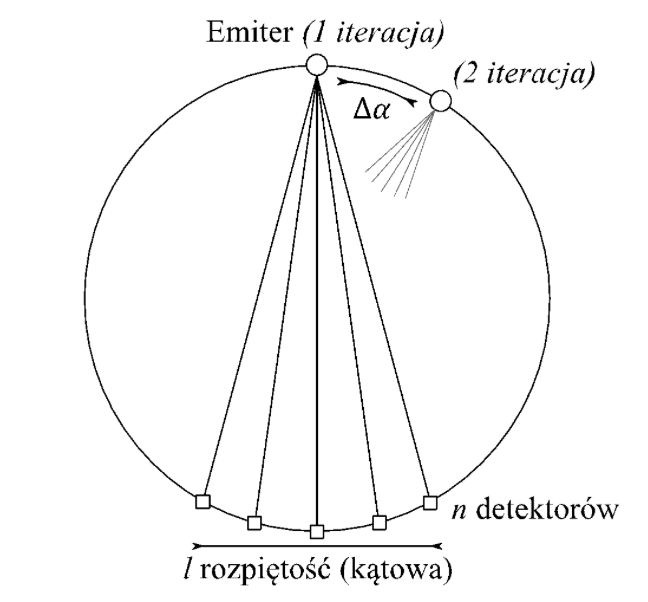
\includegraphics[scale=0.7]{img/model.png}
				\caption{model stożkowy}
			\end{figure}
		\noindent Zastosowany został model stożkowy.
		 Zakłada on wykorzystanie jednego emitera,
		  który współpracuje ze wszystkimi detektorami, tworząc wspomniany stożek 
		  (w przeciwieństwie do modelu równoległego, gdzie każdy detektor posiada własny emiter).
		
	\section{Program}
		\subsection{Środowisko}
			Do zasymulowania tomografu,
			 skorzystaliśmy z języka Python w środowisku Jupyter Notebook,
			 co pozwoliło uzyskać interfejs użytkownika niskim kosztem.
			 Skorzystaliśmy również z bibliotek, które oferowały dodatkowe funkcjonalności, m.in.:
			
			\begin{description}
				\item[numpy] funkcje i stałe matematyczne
				\item[matplotlib] wyświetlanie grafik
				\item[ipywidgets] interfejs użytkownika
				\item[pydicom] odczyt i zapis plików DICOM
				\item[cv2] zwiększenie kontrastu przefiltrowanych zdjęć
			\end{description}
			
			\subsection{Opis działania}
				\subsubsection{Sinogram}
				
				Sinogram, jest to tablica danych, 
				gdzie każdy wiersz to jedna iteracja (pozycja emitera), 
				a każda kolumna oznacza jeden detektor.
				Aby otrzymać sinogram, należy wykonać n iteracji, 
				w których emiter wraz z~detektorami będzie się stopniowo przesuwał po okręgu, 
				aż obrócimy cały układ o 360 stopni. 
				Podczas każdej iteracji wyznaczamy współrzędne punktów, w których znajduje się emiter $E$ oraz detektory $D_i$.
				\begin{center}
					\begin{tabular} {l l l}
						$ E = [ x_E, y_E ] $ 	& \hspace{2cm}	 &	$ D_i = [x_{D_i}, y_{D_i}] $
						\\
						$ x_E = r \times \cos{\alpha} $ 	& \hspace{2cm}	 &	 $ x_{D_i} = r \times \cos{\big(\alpha + \pi - \frac{\phi}{2} + i \times \frac{\phi}{n-1}\big)} $
						 \\ 
						$ y_E = r \times \sin{\alpha} $ 	& \hspace{2cm}	 &	 $ y_{D_i} =  r \times \sin{\big(\alpha + \pi - \frac{\phi}{2} + i \times \frac{\phi}{n-1}\big)}$ 
						\\
					\end{tabular}
				\end{center}
				gdzie: \\
				\indent $r$ -- połowa przekątnej obrazu, \\
				\indent $\alpha$ -- kąt przesunięcia systemu względem obrazu, \\
				\indent $\phi$ -- rozpiętość kątowa układu detektorów. \\ \\
				Wyznaczone współrzędne zakładają punkt $(0,0)$, jako środek systemu/obrazu.
				 Należy przekształcić je do układu współrzędnych obrazu,
				  gdzie punkt $(0,0)$ znajduje się w jednym z jego narożników.
				
				Aby pobrać dane z obiektu znajdującego się między emiterem a detektorami (w naszym przypadku z obrazka),
				 wykorzystujemy algorytm \textbf{Bresenhama}.
				  Służy on do wyznaczenia pikseli leżących na linii między dwoma punktami. 
				  Przechodzi iteracyjnie przez wszystkie wartości na jednej osi
				   (np. OX, jeśli obrazek jest szerszy niż wyższy).
				    W każdym kroku decyduje,
				     czy wykonać tylko ruch wzdłuż jednej osi (poziomo/pionowo), czy obu (na ukos).
				
				\begin{figure}[!h]
					\centering
					\begin{minipage}{0.4\linewidth}
						\begin{lstlisting}[language=Python, frame=single]
for i in range(x1, x2):
    points.append((i, j))
    if e > 0:
        j += m
        e += 2 * (dy - dx)
    else:
        e += 2 * dy
						\end{lstlisting}
						\caption{Fragment kodu algorytmu}
					\end{minipage}
					\hfill
					\begin{minipage}{0.45\linewidth}
						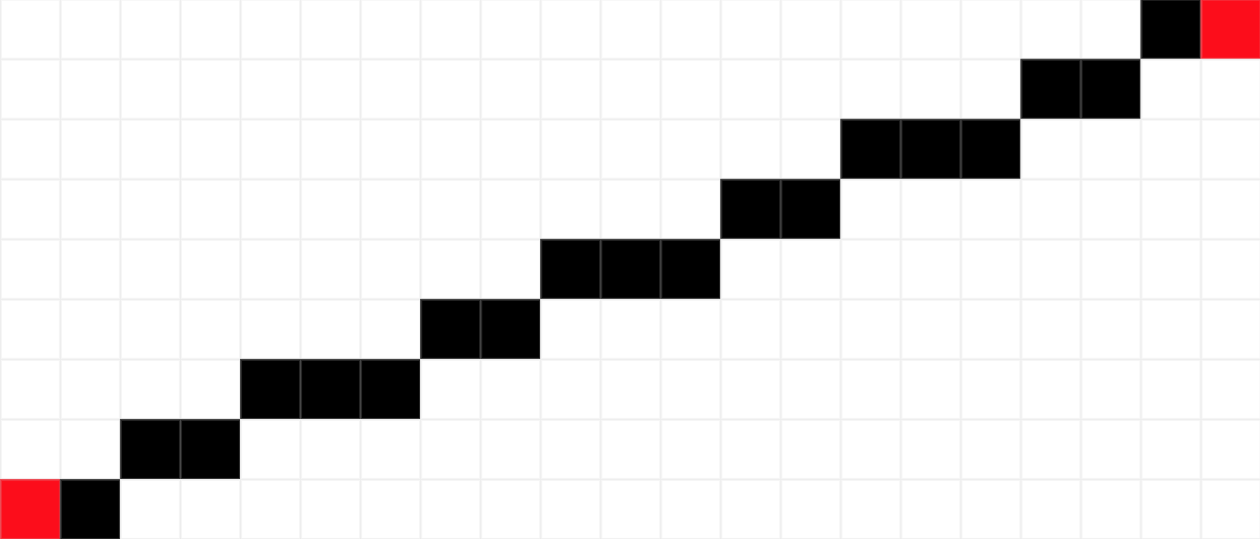
\includegraphics[width=\textwidth]{img/bresenham.png}
						\caption{Przykład działania -- znajdowanie pikseli między dwoma czerwonymi}
					\end{minipage}
				\end{figure}
				
				Znając wszystkie piksele leżące między emiterem, a detektorem, 
				sumujemy ich jasność i zapisujemy w odpowiednim miejscu sinogramu.
				Na koniec, normalizujemy wszystkie dane, tak aby wartości były z~przedziału od~0~do~1.
				 W tym celu znajdujemy największą wartość (najjaśniejszy piksel) i dzielimy przez nią pozostałe.
				
				\subsubsection{Obraz wynikowy}
					Sinogram nie jest zrozumiały dla człowieka, 
					dlatego należy go przekształcić.
					Zaczynamy od czarnego obrazu i znów przejdziemy przez n iteracji.
					Każdej iteracji będzie przypisana pozycja emitera wraz z~detektorami 
					(będą to te same pozycje, co podczas generowania sinogramu).
					Wyznaczamy linie przechodzące przez obraz między emiterem i detektorami (algorytm Bresenhama).
					Każdy piksel, przez który przechodzi linia będzie rozjaśniony o wartość odczytaną z sinogramu 
					(dla danego detektora w danej iteracji). 
					Nałożenie wszystkich linii na obrazie stworzy obraz wynikowy.
				
					\begin{figure}[!h]
						\centering
						\begin{minipage}{0.45\linewidth}
							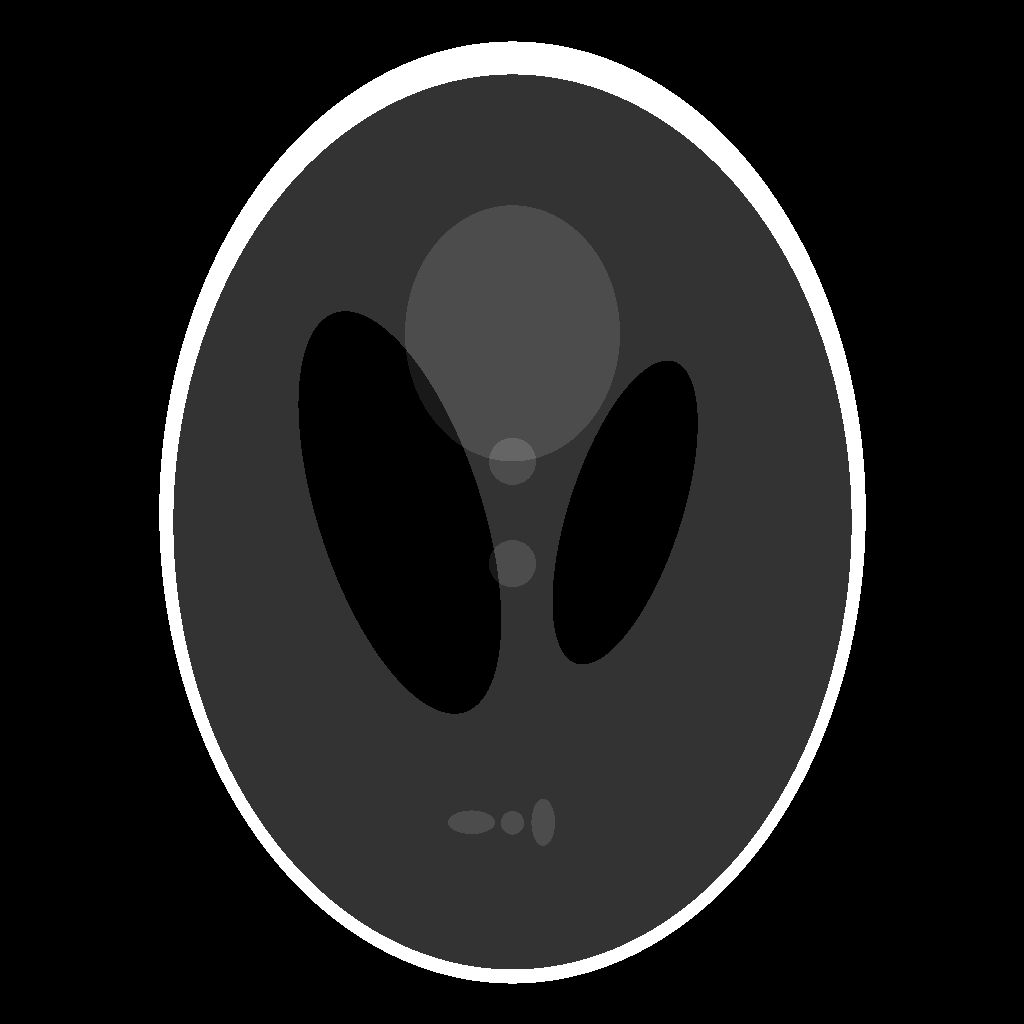
\includegraphics[width=\linewidth]{../tomograf-zdjecia/Shepp_logan.jpg} 
							\caption{obraz wejściowy}
						\end{minipage}
						\hfill
						\begin{minipage}{0.45\linewidth}
							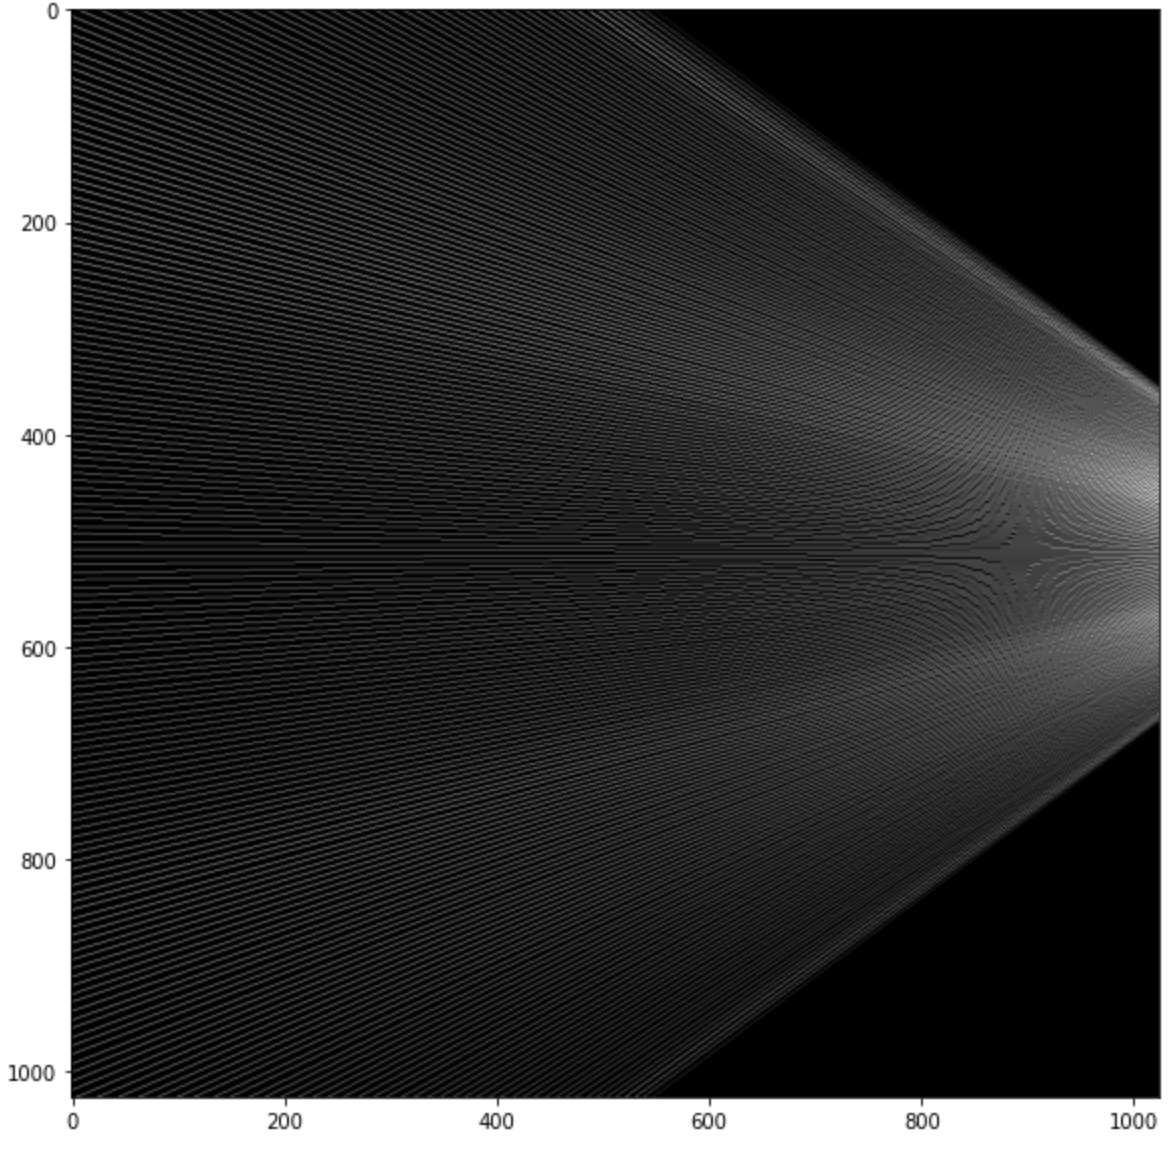
\includegraphics[width=\linewidth]{img/out_1.png}
							\caption{obraz wyjściowy -- 1. iteracja}
						\end{minipage}
					\end{figure} 
				
					\begin{figure}[!h]
						\centering
						\begin{minipage}{0.45\linewidth}
							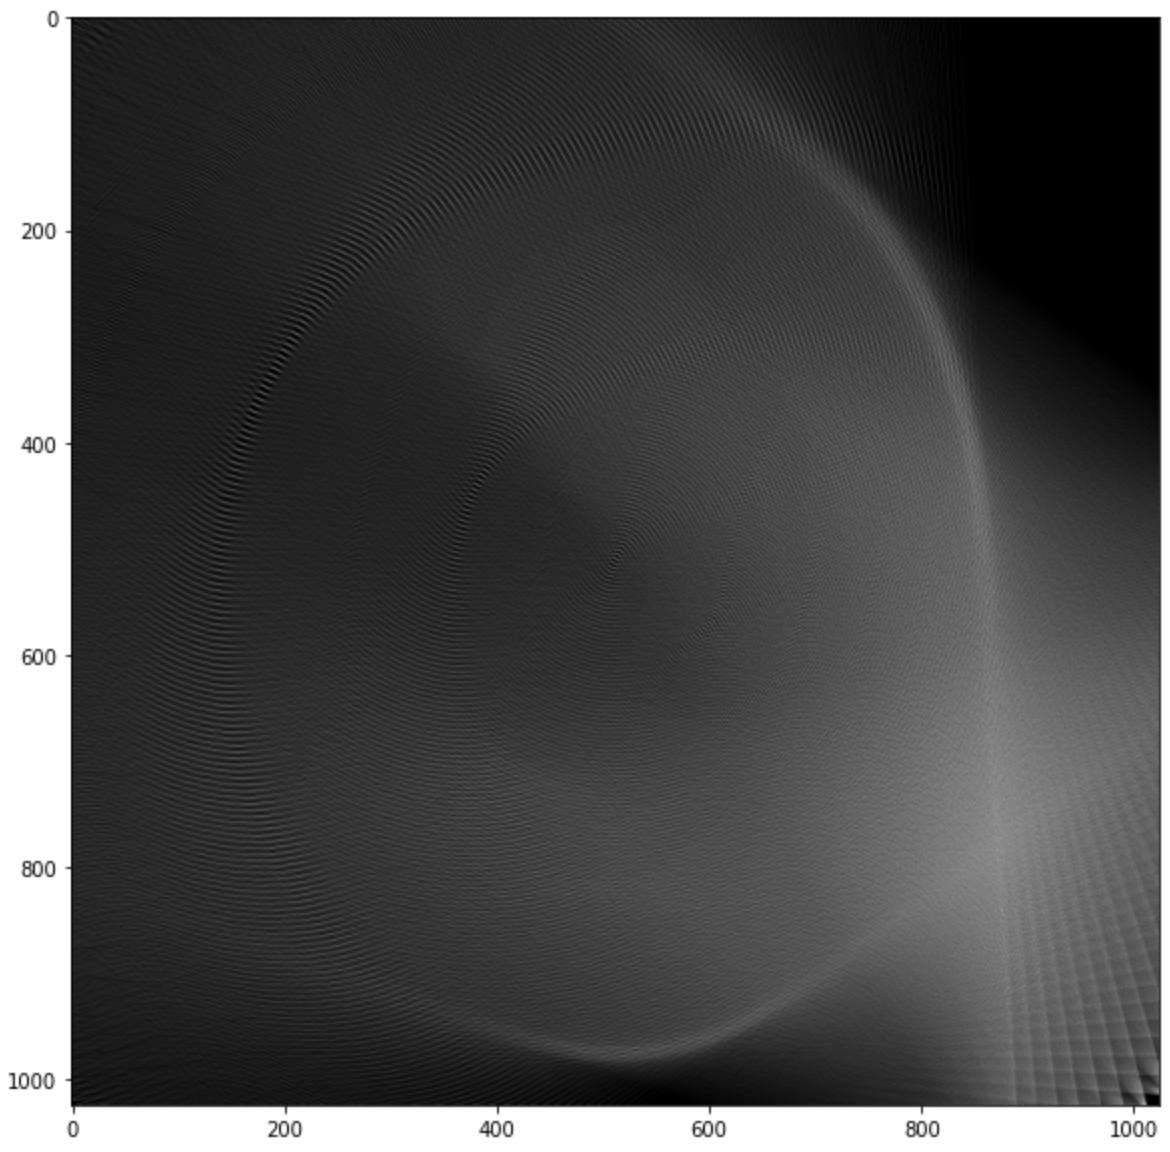
\includegraphics[width=\linewidth]{img/out_30.png}
							\caption{obraz wyjściowy -- 30. iteracja}
						\end{minipage}
						\hfill
						\begin{minipage}{0.45\linewidth}
							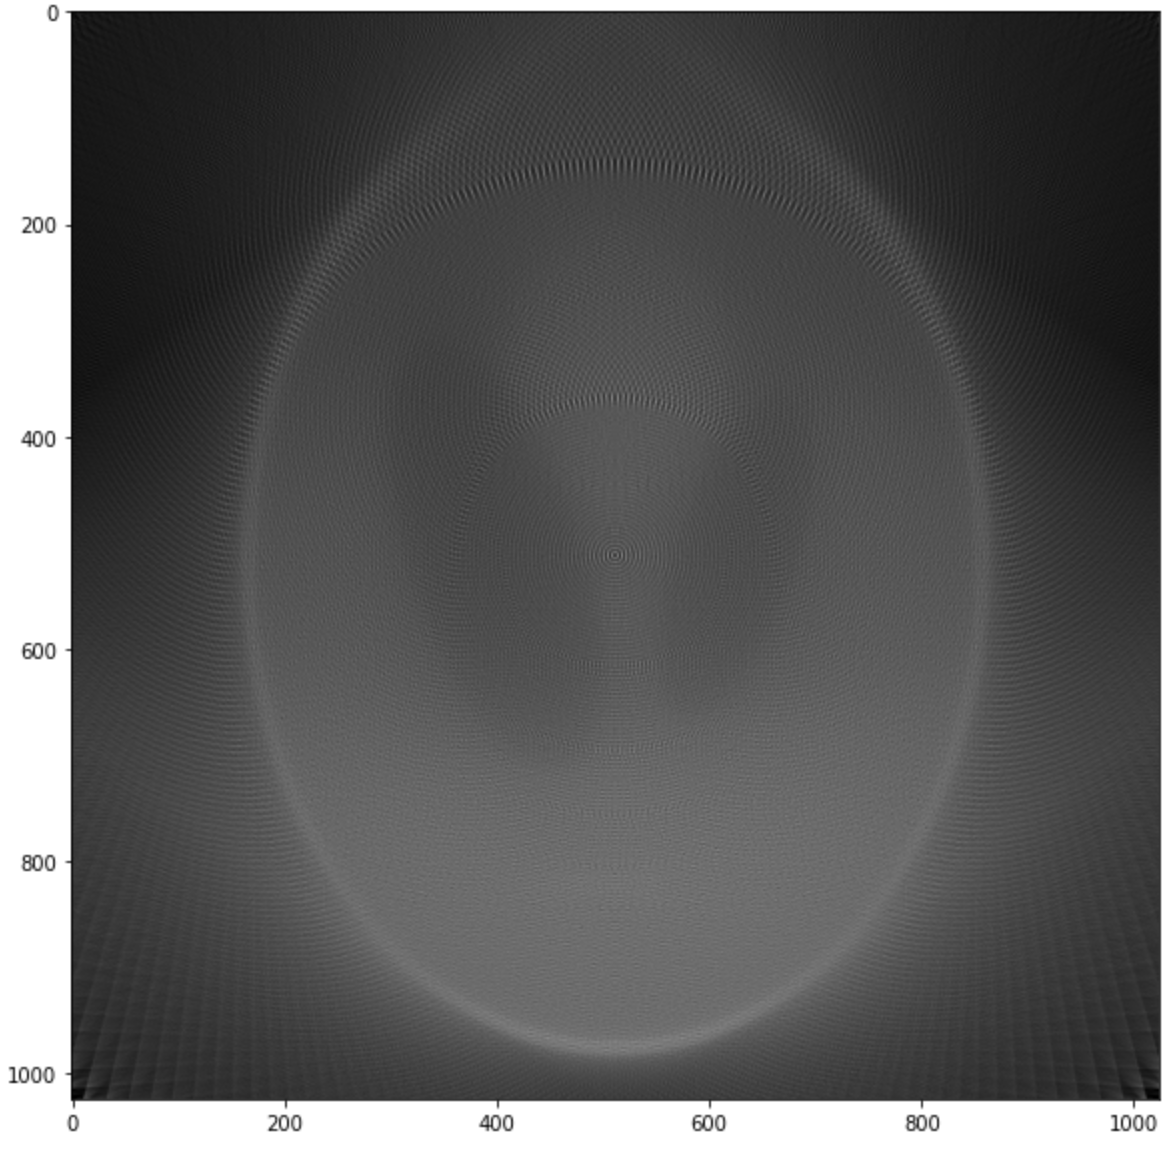
\includegraphics[width=\linewidth]{img/out_90.png}
							\caption{obraz wyjściowy -- 90. iteracja}
						\end{minipage}
					\end{figure} 
				
				\subsection{Filtr}
					Obraz wynikowy jest w znaczącym stopniu rozmyty.
					Aby temu zapobiec, należy każdy dodatni sygnał z detektorów otoczyć ujemnymi wartościami.
					\begin{figure}[!h]
					\centering
						\begin{lstlisting}[language=Python, frame=single]
iteracja_freq = fft.rfft(iteracja)
filtr = np.floor(np.arange(0.5, len(iteracja)//2 + 0.1, 0.5 ))
out_freq = iteracja_freq * filtr
out = fft.irfft(out_freq)
						\end{lstlisting}
						\caption{fragment kodu filtrującego}
				\end{figure}
					
					Dane z detektorów przekształcamy do dziedziny częstotliwościowej,
					 mnożymy przez filtr, 
					 po czym wracamy do dziedziny przestrzennej.
					Obraz po filtracji znacząco zyska na ostrości, lecz utraci na rozpiętości tonalnej.
					Z tego powodu przepuszczamy go przez funkcję zwiększającą kontrast.
					
					\begin{figure}[!h]
						\centering
						\begin{minipage}{0.45\linewidth}
							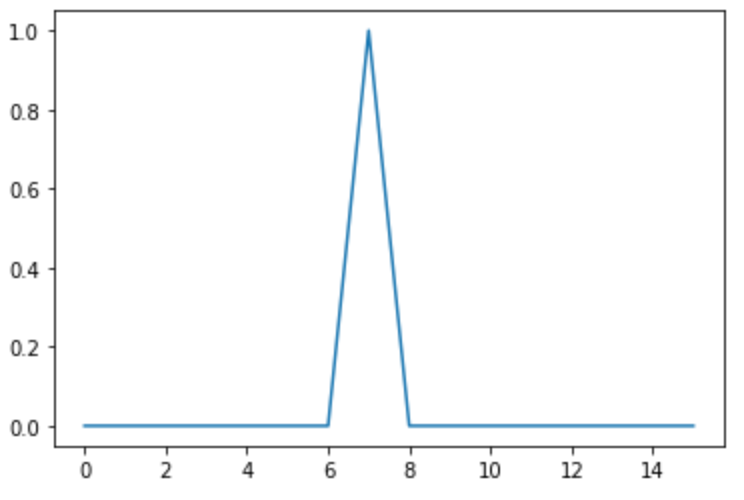
\includegraphics[width=\linewidth]{img/filtr_1.png}
							\caption{przykładowe dane z detektorów}
						\end{minipage}
						\hfill
						\begin{minipage}{0.45\linewidth}
							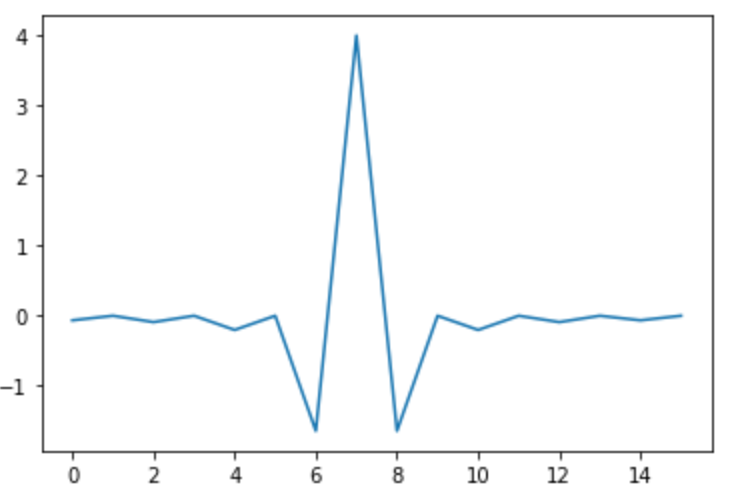
\includegraphics[width=\linewidth]{img/filtr_2.png}
							\caption{dane z detektorów po przefiltrowaniu}
						\end{minipage}
					\end{figure}
			
			
			\subsection{Standard DICOM}
			Wyniki zapisujemy w standardzie DICOM. 
			Do jego obsługi używamy biblioteki \texttt{pydicom}.
			W pliku, oprócz samego skanu, zapisujemy też dane pacjenta (imię i nazwisko, płeć, datę urodzenia), komentarze, datę i czas badania.
			Wykorzystujemy w tym celu następujące pola:
			\begin{figure}[!h]
				\centering
				\begin{tabular}{|c|c|c|}
				\hline
				\textbf{Identyfikator pola} & \textbf{Nazwa pola} & \textbf{Opis} \\
				\hline \hline
				(0008, 0023) & Content Date & data badania \\
				\hline
				(0008, 0033) & Content Time & czas badania \\
				\hline
				(0010, 0010) & Patient's Name & imię i nazwisko pacjenta \\
				\hline
				(0010, 0030) & Patient's Birth Date & data urodzenia pacjenta \\
				\hline
				(0010, 0040) & Patient's Sex & płeć pacjenta \\
				\hline
				(0010, 4000) & Patient Comments & komentarze \\
				\hline
				(0028, 0010) & Rows & liczba wierszy obrazka (wysokość) \\
				\hline
				(0028, 0011) & Columns & liczba kolumn obrazka (szerokość) \\
				\hline
				(7fe0, 0010) & Pixel Data & obrazek (piksele) \\
				\hline
				\end{tabular}
				\caption{Niektore z wykorzystanych pól}
			\end{figure}
			\newpage
			Fragment kodu odpowiedzialnego za zapis pokazuje rysunek \ref{dicomsave}. Do odczytu pliku skorzystaliśmy z funkcji \texttt{pydicom.dcmread(filename)}, która pozwala następnie na dostęp do wszystkich pól z pliku.
			
			\begin{figure}[!h]
				\centering
				\begin{lstlisting}[language=Python, frame=single]
ds = FileDataset(filename, {}, file_meta=file_meta, preamble=b"\0" * 128)
ds.PatientName = name
ds.PatientSex = sex
ds.PatientBirthDate = birth.strftime('%Y%m%d')
ds.PatientComments = comment

ds.ContentDate = date.strftime('%Y%m%d')
ds.ContentTime = date.strftime('%H%M%S.%f')

# 1 lub 3 - ile kolorow na obrazie
ds.SamplesPerPixel = 1
# interpretacja (MONOCHROME, RGB, HSV, ...)
ds.PhotometricInterpretation = "MONOCHROME2"
# 0 - unsigned int, 1 - U2
ds.PixelRepresentation = 0
# najwyzszy bit
ds.HighBit = 15
# ilosc bitow na piksel
ds.BitsStored = 16
# ilosc bitow zaalokowanych na piksel
ds.BitsAllocated = 16
# minimalna wartosc piksela - 0
ds.SmallestImagePixelValue = str.encode('\x00\x00')
# maksymalna wartosc piksela - ffff?
ds.LargestImagePixelValue = str.encode('\xff\xff')
# kolumny, wiersze i dane
ds.Columns = image.shape[1]
ds.Rows = image.shape[0]
ds.PixelData = (image * 65535).astype('uint16').tobytes()

ds = correct_ambiguous_vr(ds, True)
ds.save_as(filename, write_like_original=False)
				\end{lstlisting}
				\caption{Fragment kodu -- zapis do pliku DICOM}
				\label{dicomsave}
			\end{figure}
			
	\section{Eksperyment}
		Korzystając z miary RMSE sprawdzimy, 
		jak poszczególne parametry wpływają na jakość obrazu wyjściowego. 
		Miara ta oblicza średnią różnicę koloru dla każdego piksela, w porównaniu do obrazu wejściowego (mniej -- lepiej). 
		Do sprawdzenia wpływu parametrów, skorzystaliśmy z obrazu \texttt{Shepp\_logan.jpg} (Rysunek 4.).
		
		\newpage
		\subsection{Wpływ parametrów na jakość obrazu}
		
		
		\begin{figure}[!h]
			\begin{minipage}{0.48\linewidth}
				\begin{tikzpicture}
					\begin{axis}[xlabel=Liczba detektorów (bez filtowania), ylabel=RMSE, only marks, xtick distance=90]
					\addplot coordinates {
						(	90	,	0.19766641872181315	)
						(	180	,	0.21241692941458212	)
						(	270	,	0.26905462144543296	)
						(	360	,	0.3185885394517024	)
						(	450	,	0.3639450780220456	)
						(	540	,	0.4146778824868383	)
						(	630	,	0.4395340917953436	)
						(	720	,	0.4303860322190707	)
					};
					\end{axis}
				\end{tikzpicture}
			\end{minipage}
			\hfill
			\begin{minipage}{0.48\linewidth}
				\begin{tikzpicture}
					\begin{axis}[xlabel=Liczba detektorów (z filtowaniem), ylabel=RMSE, only marks, xtick distance=90]
					\addplot coordinates {
						(	90	,	0.47944557897904283	)
						(	180	,	0.4672745431104078	)
						(	270	,	0.46244981936422036	)
						(	360	,	0.4574380736275415	)
						(	450	,	0.4548210642769736	)
						(	540	,	0.4520704744176787	)
						(	630	,	0.4501465702251961	)
						(	720	,	0.4484138396604839	)
					};
					\end{axis}
				\end{tikzpicture}
			\end{minipage}
		\end{figure}
		
		\begin{figure}[!h]
			\centering
			\begin{minipage}{0.48\linewidth}
				\begin{tikzpicture}
					\begin{axis}[xlabel=Liczba skanów, ylabel=RMSE, only marks, xtick distance=90]
					\addplot coordinates {
						(	90	,	0.2174929558603675	)
						(	180	,	0.21241692941458212	)
						(	270	,	0.20935852709603195	)
						(	360	,	0.2082807671066534	)
						(	450	,	0.20821266152493592	)
						(	540	,	0.20863697322807373	)
						(	630	,	0.20817212780354352	)
						(	720	,	0.2069512394127205	)
					};
					\end{axis}
				\end{tikzpicture}
			\end{minipage}
			\hfill
			\begin{minipage}{0.48\linewidth}
				\begin{tikzpicture}
					\begin{axis}[xlabel={Rozpiętość wachlarza [°]}, ylabel=RMSE, only marks, xtick distance=45]
					\addplot coordinates {
						(	45	,	0.2362	)
						(	90	,	0.2195	)
						(	135	,	0.2471	)
						(	180	,	0.2124	)
						(	225	,	0.2091	)
						(	270	,	0.211	)
					};
					\end{axis}
				\end{tikzpicture}
			\end{minipage}
			
		\end{figure}
				
		W wersji bez filtrowania, błąd rośnie wraz z wzrostem \textbf{liczby detektorów}.
		Wynika to z faktu, że ilość detektorów wpływa na jasność obrazu wyjściowego (więcej -- jaśniej).
		 Nie występuje to w wersji z filtrem,
		  ponieważ kompensujemy tę jasność dodatkowymi ujemnymi wartościami.
		 Podczas oglądania wynikowych obrazów można jednoznacznie stwierdzić, 
		 że większa liczba detektorów powoduje zwiększenie jakości obrazu.
		 Warto nadmienić, że zbyt mała liczba detektorów wpływa na powstawanie defektów w postaci kręgów. 
		
		
		Zwiększenie \textbf{liczby skanów} ma pozytywny wpływ na jakość obrazu wynikowego.
		Gdy jest ich więcej, mniej widoczne stają się linie biegnące ze środka obrazu do zewnątrz, a także sam środek jest bardziej wyraźny, ma mniej defektów.
		
		Zastosowanie większej \textbf{rozpiętości wachlarza} również pozwala na zmniejszenie różnicy między obrazem wyjściowym, a oryginałem.
		Bardzo mała rozpiętość powoduje, że wynik zdecydowanie odbiega od oczekiwań -- nie przypomina w żadnym stopniu obrazu wejściowego.
		
		\newpage
		\subsection{Porównanie obrazu z filtrem i bez}
			\begin{figure}[!h]
				\centering
				\begin{minipage}{0.45\linewidth}
					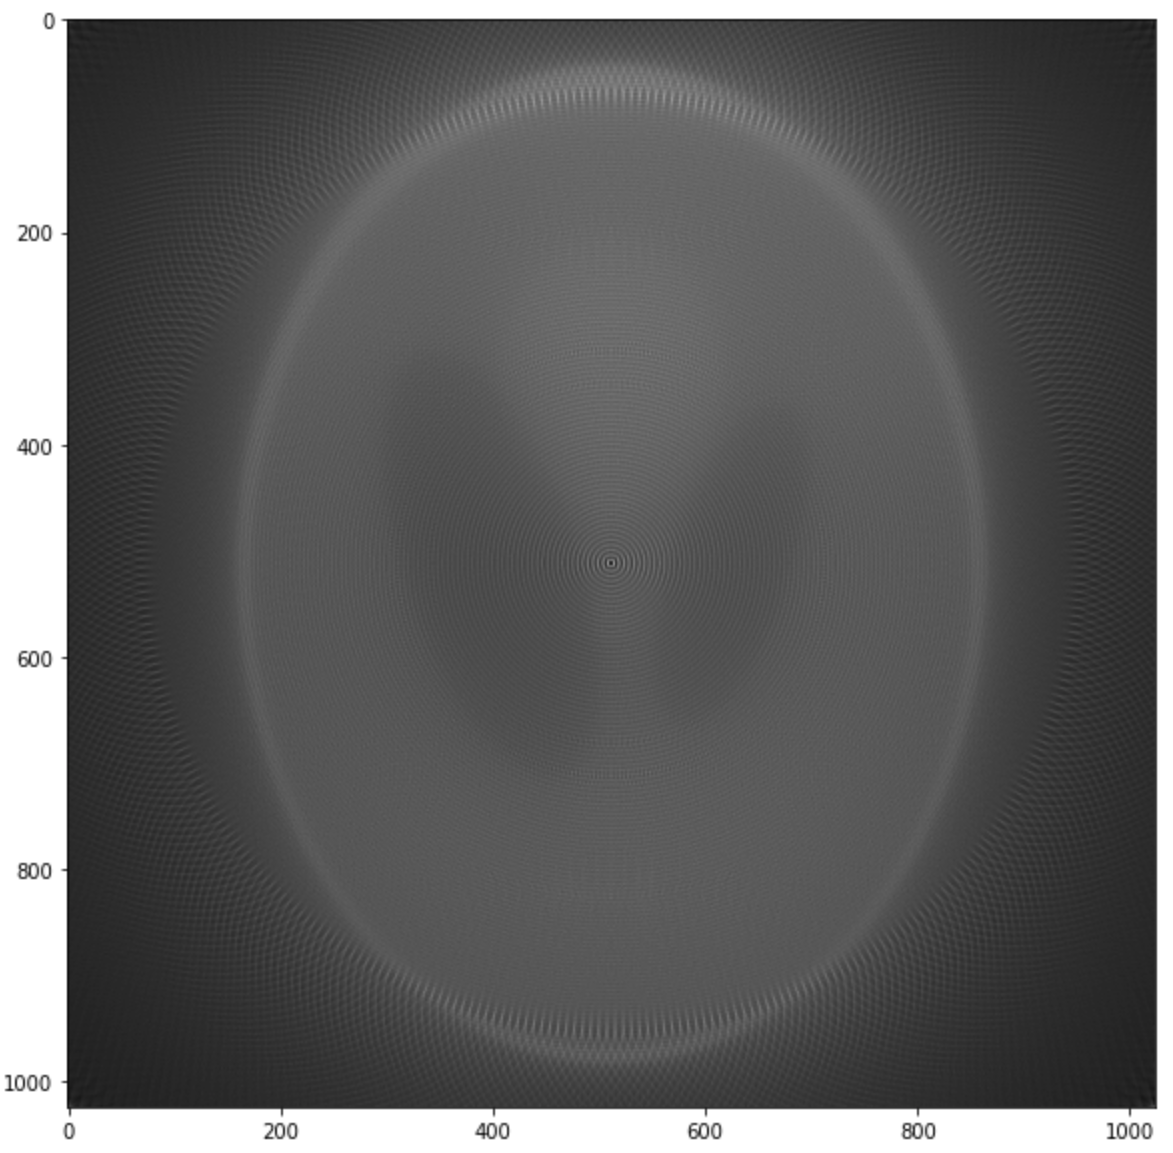
\includegraphics[width=\linewidth]{img/shepp_nf.png}
					\caption{wynik bez filtracji, RMSE -- 0.25}
				\end{minipage}
				\hfill
				\begin{minipage}{0.45\linewidth}
					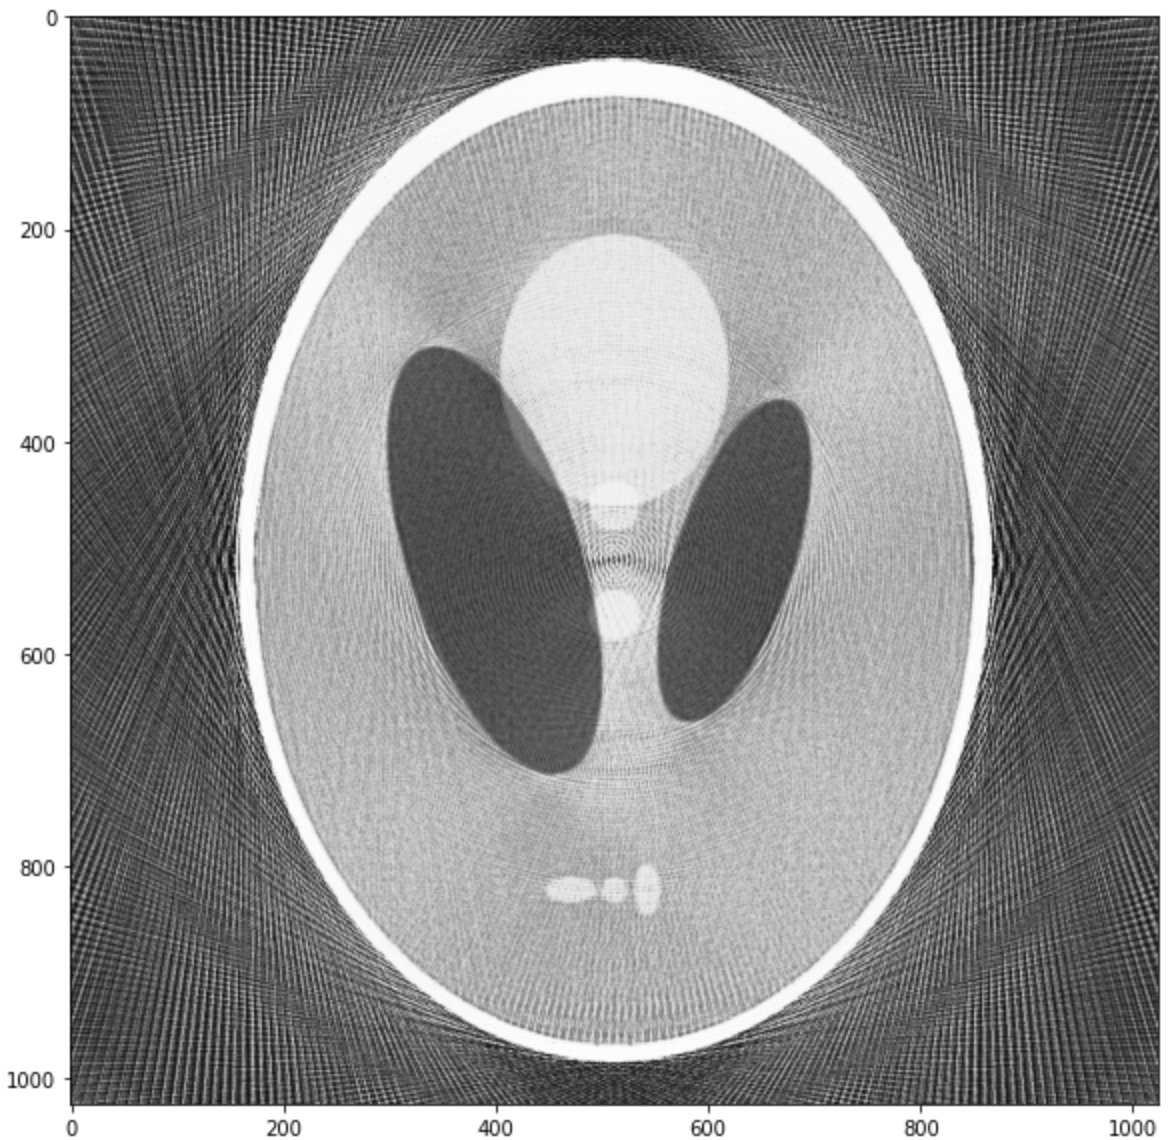
\includegraphics[width=\linewidth]{img/shepp_f.png}
					\caption{wynik z filtrem, RMSE -- 0.46}
				\end{minipage}
			\end{figure}
			
			\begin{figure}[!h]
				\centering
				\begin{minipage}{0.45\linewidth}
					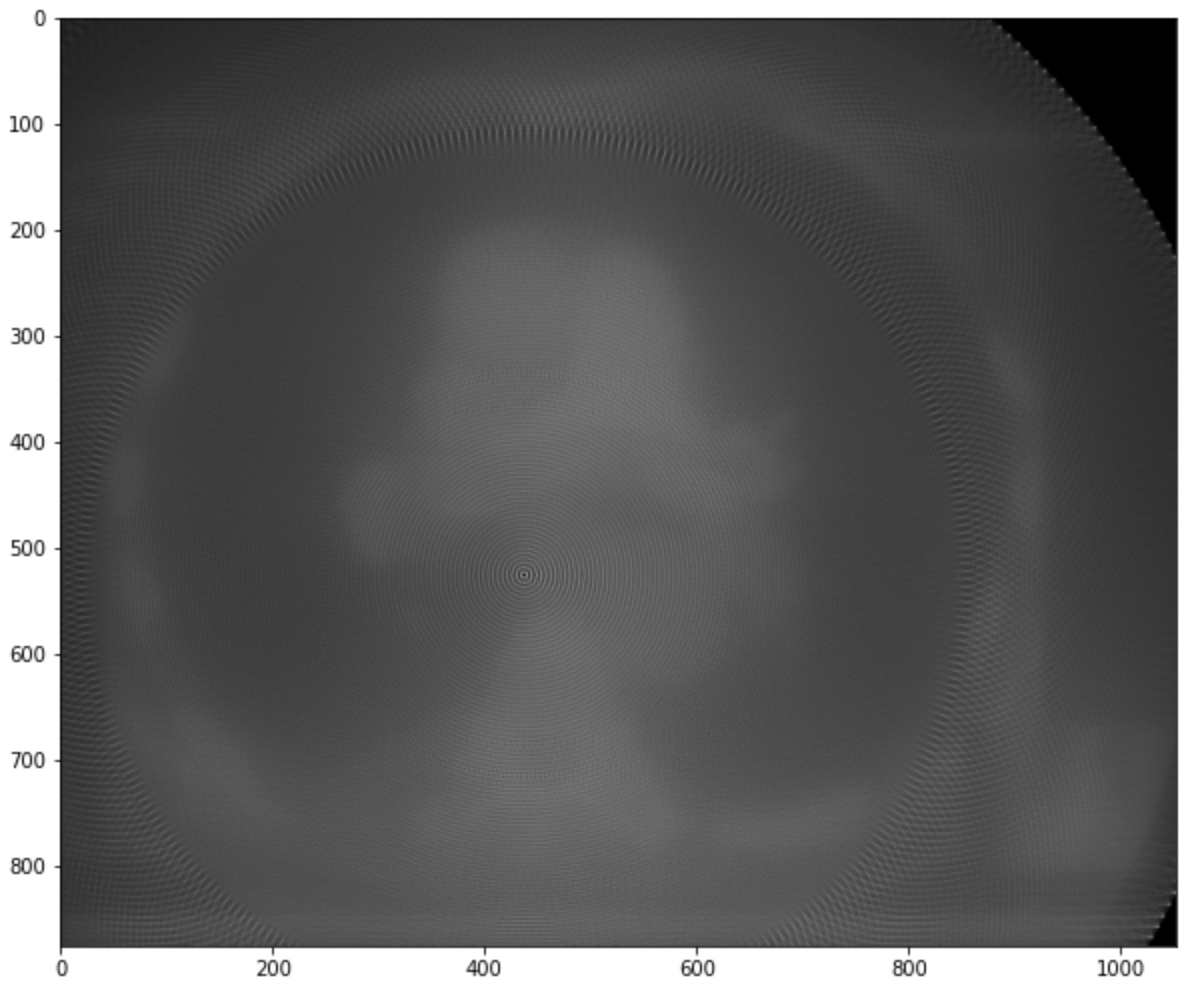
\includegraphics[width=\linewidth]{img/saddle_nf.png}
					\caption{wynik bez filtracji, RMSE -- 0.31}
				\end{minipage}
				\hfill
				\begin{minipage}{0.45\linewidth}
					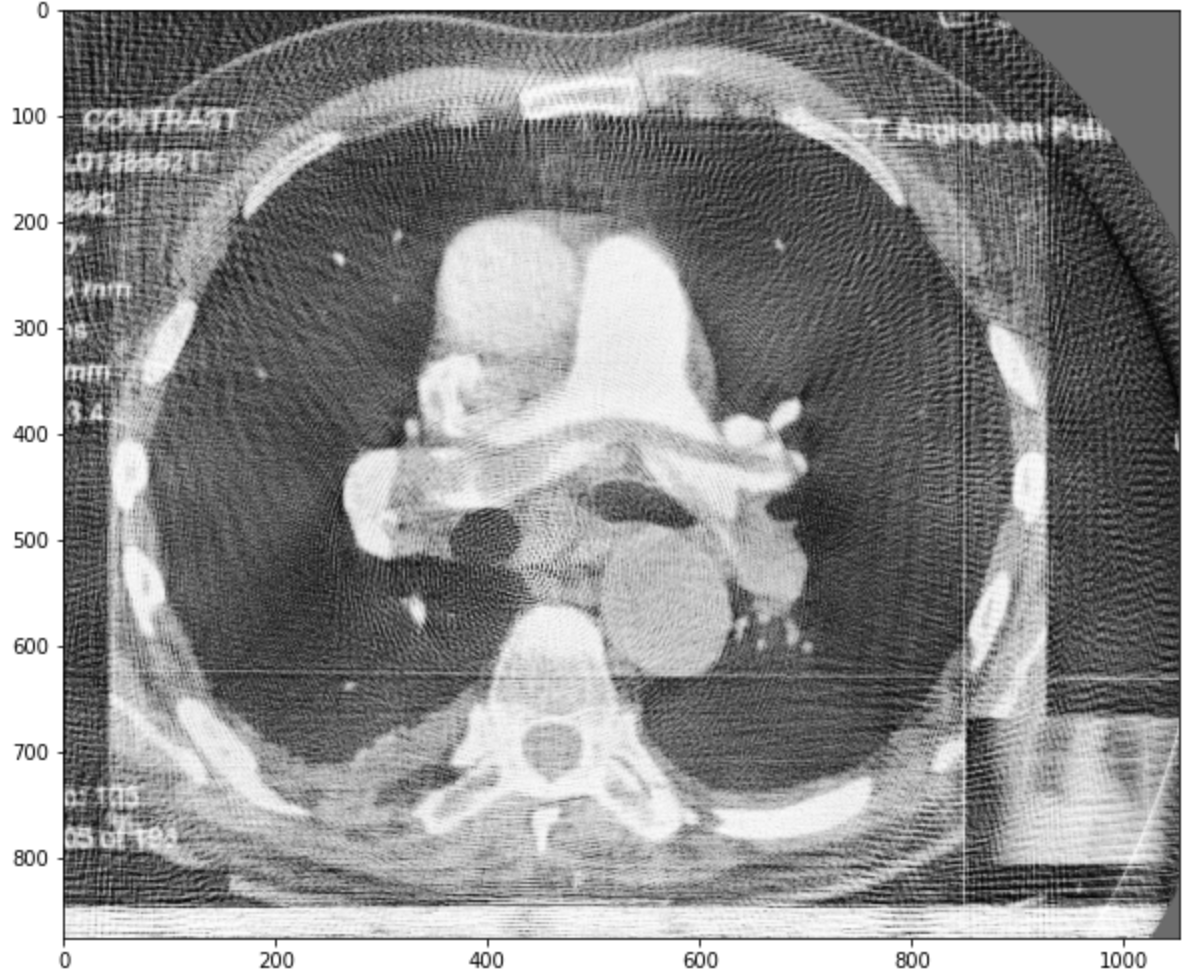
\includegraphics[width=\linewidth]{img/saddle_f.png}
					\caption{wynik z filtrem, RMSE -- 0.33}
				\end{minipage}
			\end{figure}
			
			Różnica w jakości obrazów jest znacząca. 
			Obrazy wyprodukowane przy użyciu filtra są wyraźne i szczegółowe. 
			Miara jakości RMSE faworyzuje obrazy bez filtracji. 
			Wynika to z faktu, że obrazy z filtrem, mimo swojej dokładności, 
			mają większą różnicę w jasności względem oryginalnego obrazu. 
			Obrazy bez filtra, mimo bycia rozmazanymi, 
			średnio bardziej odpowiadają oryginałowi. 
			Ponadto, filtracja wprowadza artefakty w postaci jasnych linii, 
			szczególnie widocznych na ciemnym tle.
			
\end{document}
